\documentclass[10pt,a4paper]{article}
\usepackage{tabu}
\usepackage{amsmath}
\usepackage{amsfonts}
\usepackage{amssymb}
\usepackage{makeidx}
\usepackage{graphicx}
\usepackage[backend=biber]{biblatex}
\usepackage{textcomp}
\DeclareMathSizes{12}{30}{16}{12}
\usepackage[margin= 1in]{geometry}
\graphicspath{ {Images/} }
\usepackage{listings}
\usepackage{float}
\addbibresource{bibliography.bib}
\usepackage{color}

\author{James Walker-Wilson}
\title{Sound Level Meter}
\makeindex
\definecolor{codegreen}{rgb}{0,0.6,0}
\definecolor{codegray}{rgb}{0.5,0.5,0.5}
\definecolor{codepurple}{rgb}{0.58,0,0.82}
\definecolor{backcolour}{rgb}{0.95,0.95,0.92}
 
\lstdefinestyle{mystyle}{
    backgroundcolor=\color{backcolour},   
    commentstyle=\color{codegreen},
    keywordstyle=\color{blue},
    numberstyle=\tiny\color{codegray},
    stringstyle=\color{black},
    basicstyle=\footnotesize,
    breakatwhitespace=false,         
    breaklines=true,                 
    %captionpos=b,                    
    keepspaces=true,                 
    numbers=left,                    
    numbersep=5pt,                  
    showspaces=false,                
    showstringspaces=false,
    showtabs=false,                  
    tabsize=2
}
 
\lstset{style=mystyle}
\begin{document}
\maketitle
\newpage

\begin{abstract}

\end{abstract}

\section{Introduction}
This report outlines the design and construction of a sound level meter. The device measures the sound level of the environment. This is the filtered through several filter stages and the sound level is displayed on an LED bar graph. The sound signal is filtered to select a band of frequencies and then low pass filtered to produce a DC voltage level proportional to the sound level.  

\subsection{Aims}
\begin{itemize}
  \item To understand the design of a common emitter amplifier for the first stage.
  \item To understand the design of an LC band pass filter.
  \item To understand the construction and operation of a signal rectifier.
  \item To understand the construction of a low pass filter.
  \item To understand how to program a PIC Micro controller.
  \item To understand the construction and testing of the circuit.  

  \end{itemize}

\subsection{Objectives}
\begin{itemize}
  \item To determine the $\beta$ of the transistor by experimentation
  \item To design a common emitter amplifier for the first stage of the circuit with appropriate gain
  \item To design an LC band pass filter and calculate the number of turns of wire to create the required inductance.
  \item To construct a rectifier to rectify the signal
  \item To construct a low pass filter to convert the signal to a dc voltage level.
  \item To create a program to change the number of LED's that are on depending on the sound level and program the Micro controller with the code.
  \item To test the completed stages and whole circuit to make sure it operates as intended.  

  \end{itemize}

\section{Method}

\subsection{Design}
\subsubsection{Determining $\beta$}
To determine $\beta$ the circuit shown in figure \ref{Beta}. $R_C$ was set to $3.9K\Omega$. $R_B$ was then chosen to make $V_{CE}\approx 7.5V$. The base current was calculated by measuring the voltage across $R_B$ and using Ohms law, the same was done for the collector current. To work out $\beta$ the formula
\begin{center}
\Huge
$\beta = \frac{I_C}{I_B}$
\end{center}
was used. This gave a value of $\beta = 337$.

\begin{figure}[!h]
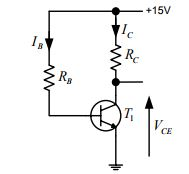
\includegraphics[scale=0.7]{beta}
\caption{Circuit used to determine $\beta$}
\label{Beta}
\end{figure}
\newpage
\subsubsection{Common Emitter Amplifier}
The first stage of the circuit is a common emitter amplifier to amplify the signal from the microphone to be processed by later stages. The transistor $\beta$ was found to be $\beta = 337$. First the current $I_C$ was calculated using the equation with $V_C = 7.5V$ and $ R_3 = 3.9K\Omega$ \newline
\begin{center}
\Huge
$I_c = \frac{15-V_c}{R_3}$
\end{center}
This equation gives an $I_c$ value of $ I_c = 1.92mA$. $R_4$ is then calculated with the equation
\begin{center}
\Huge
$R_4 = \frac{1.5}{I_E}$
\end{center}
with $I_e \approx I_c$ this makes $R_4= 781 \Omega$. To calculate the biasing resistors it is set that the current through the biasing resistors is $10\times I_B$. The equation 
\begin{center}
\Huge
$R_2 = \frac{V_{BE} + V_E}{10\times I_B}$
\end{center}
This gives an $R_2 \approx 40K\Omega$
$R_1$ can then be calculated with the equation.
\begin{center}
\Huge
$R_1 = \frac{V_{CC}-V_B}{10\times I_B}$
\end{center} 
This gives $R_1 \approx 27K\Omega$
\begin{figure}
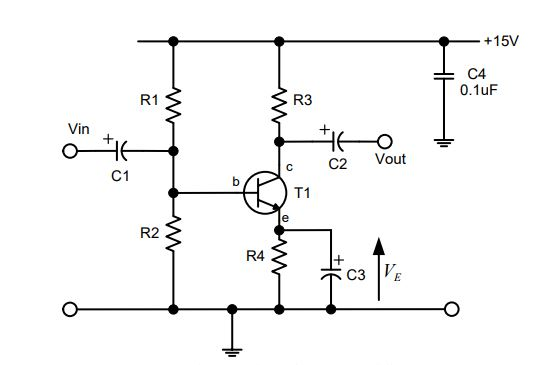
\includegraphics[scale=1]{CircuitDiagram}
\caption{Common emitter amplifier circuit diagram}
\end{figure}

\subsubsection{Bandpass Filter}
The band pass filter uses a resonant LC circuit to set the filter characteristics. The resonant frequency of an LC circuit is given as 

\begin{center}
\Huge

$f = \frac{1}{2\pi\sqrt{LC}}$

\end{center}

The capacitor that forms the resonant circuit is $C5 = 1\mu F$
to calculate the value for $L$ the equation is rearranged to 
\begin{center}
\Huge

$L = \frac{1}{(2\pi f)^2 C}$

\end{center}
This gives $L = 11.3mH$. To calculate the number of turns on the inductor the equation

\begin{center}
\Huge

$N= \sqrt{\frac{Ll}{\mu \times a}}$
\normalsize
\newline
$L=$ Inductance,$l=$ length of magnetic circuit,$\mu=$ permeability and $a=$ cross sectional area. 

\end{center}


is used. This gives $N=61$ Turns.

\begin{figure}[!h]
\label{BPF}
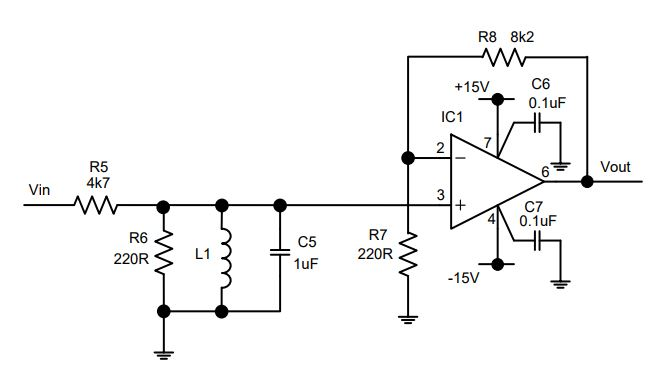
\includegraphics[width= \textwidth]{Bandpass}
\caption{Band pass filter circuit diagram}

\end{figure}
\subsubsection{Code}
The code was made to light all the LED's when maximum sound level was achieved. This was done with a logarithmic scale to allow high sensitivity at low sound levels but allow a large range of sound levels to be measured without clipping at high end values.

\begin{tabu} to 0.8\textwidth { | X[c] | X[c] |}
 \hline
 Number of bars lit & Voltage level(mV)\\
 \hline
 0 & 0\\
 \hline
 1 & 1.8\\
 \hline
 2 & 3.28\\
 \hline
 3 & 5.94\\
 \hline
 4 & 10.76\\
 \hline
 5 & 19.49\\
 \hline
 6 & 35.3\\
 \hline
 7 & 63.95\\
 \hline
 8 & 115.8\\
 \hline
 9 & 209\\
 \hline
 10 &380\\
 \hline

\end{tabu}
\newline
These values were then used to create the code 
\begin{lstlisting}[caption={PIC Code},label={lst:code},language= C]
//Newcastle University - EEE - Stage 1 - Sound Level Meter
//16F819 PIC software to drive a 10-LED bargraph display from a dc level on ADC input 0 (AN0).
//Port A and B used to drive LEDs.
//Pin Configuration:
//Pin Configuration:
//1-RA2 (LED4) 18-NC
//2-RA3 (LED3) 17-AN0 (DC Sound Level input)
//3-NC 16-RA7 (LED1)
//4-MCLR 15-RA6 (LED2)
//5-VSS 14-VDD
//6-RB0 (LED10) 13-RB7 (PGD)
//7-RB1 (LED9) 12-RB6 (PGC)
//8-RB2 (LED8) 11-RB5 (LED5)
//9-RB3 (LED7) 10-RB4 (LED6)
#include <xc.h> //header file for device
#include <stdint.h> //header file for standard types e.g uint8_t
//fuse settings to configure device
//i.e. NOWDT - No Watchdog Timer, INTOSCIO - Internal clock used, pins available for I/O
#pragma config MCLRE = ON, CP = OFF, CPD = OFF, BOREN = OFF, WDTE = OFF
#pragma config PWRTE = OFF, FOSC = INTOSCIO, LVP = OFF, DEBUG = ON
void main()
{
 //*** INSERT ANY VARIABLE DECLARATIONS HERE ***
 //uint8_t = 8-bit unsigned number
 //unint16_t = 16-bit unsigned number
 uint16_t value;
 //*** The following code initializes the PIC ***
 OSCCONbits.IRCF = 0b111; //use internal 8MHz clock (FOSC=8MHz)
 TRISB = 0b00000000; //Port B all outputs
 TRISA = 0b00110011; //Port A B6/B7/B3/B2 outputs
 ADCON1bits.ADFM = 1; //A/D Result Format Right Justified
 ADCON1bits.ADCS2 = 1; //A/D clock Source divided by 2
 ADCON1bits.PCFG = 0b1110; //Enable AN0 input for sound level ADC
13
 ADCON0bits.ADCS = 0b01; //set ADC clock, should be between 1.6us and 6.4us (1/8MHz x 16 = 2us)
 ADCON0bits.CHS = 0b000; //select AN0 for input
 ADCON0bits.ADON = 1; //A/D Converter is operating
 do
 {
 //The code below will read the digital value from the 10-bit analogue to digital converter.
 //The range of the return value will be between 0 and 1023. Where 0V = 0 and 5V = 1023.
 //For example 2.5V on the ADC will return 511 to the variable value below.
 ADCON0bits.GO_nDONE = 1; //start A/D conversion
 while(ADCON0bits.GO_nDONE == 1); //wait for A/D conversion to complete
 value = ADRESH; //read MSB of ADC result
 value = value << 8; //shift left 8 bits
 value = value + ADRESL; //read LSB of ADC result. value now contains a 10-bit ADC number
 //*** INSERT YOUR PROGRAM CODE HERE TO ILLUMINATE THE LEDs***
 //The basic requirement of your code is:-
 //(i) To use the variable value to determine which LED bars should be switched on.
 //(ii) To write the appropriate code to the output pins RB0-RB5 and RA2,RA3,RA6,RA7.
 //The PIC PORTA and PORTB registers should be used to output a value to the Port pins
 //PORTA=0b00001111; will output a binary number to port A. Bits 7,6,5,4=0 and Bits 3,2,1,0=1.
 //Alternatively PORTA=15; for decimal equivalent.
 //The parameter may also be a variable instead of a constant e.g. PORTA=value;
 
if(value = 0){
PORTA=0b11111111
PORTB=0b11111111

}  
 
if(value > 0 && value <= 1.8){
PORTA=0b01111111
PORTB=0b11111111

} 

if(value > 1.8 && value <= 3.28){
PORTA=0b00111111
PORTB=0b11111111

} 

if(value > 3.28 && value <= 5.94){
PORTA=0b00110111
PORTB=0b11111111

} 

if(value > 5.94 && value <= 10.76){
PORTA=0b00110011
PORTB=0b11111111

} 

if(value > 10.76 && value <= 19.49){
PORTA=0b00110011
PORTB=0b11011111

} 

if(value > 19.49 && value <= 35.3){
PORTA=0b00110011
PORTB=0b11001111

} 

if(value > 35.3 && value <= 63.95){
PORTA=0b00110011
PORTB=0b11000111

}

if(value > 63.95 && value <= 115.8){
PORTA=0b00110011
PORTB=0b11000011

}

if(value > 115.8 && value <= 209){
PORTA=0b00110011
PORTB=0b11000001

}

if(value > 115.8 && value <= 209){
PORTA=0b00110011
PORTB=0b11000001

}




 
 
 
 
 
 
 } while (1);
}

\end{lstlisting}

\subsection{Construction}
\subsubsection{Common Emitter Amplifier}
After the common emitter amplifier was constructed on bread board using the resistor values determined in the design stage. This was to determine that the amplifier had been designed correctly. To test the design the voltage between the transistor collector and ground was measured and was found to be $V_C = 7.62V$. This is within the allowable limit of $6V$ to $9V$. The circuit was then constructed on the circuit board and the collector voltage was once again measured and found to be the same as before. The decoupling capacitors were then added to the circuit board. To test the amplifier a $20mV Pk-Pk$ sine wave at $1kHz$ was applied to the input and the output measured on an oscilloscope. This is shown in figure \ref{CEE}. Using an input of $23mV$ and an output of $4.3V$ leads to a gain of $G= 215$.

\begin{figure}[!h]



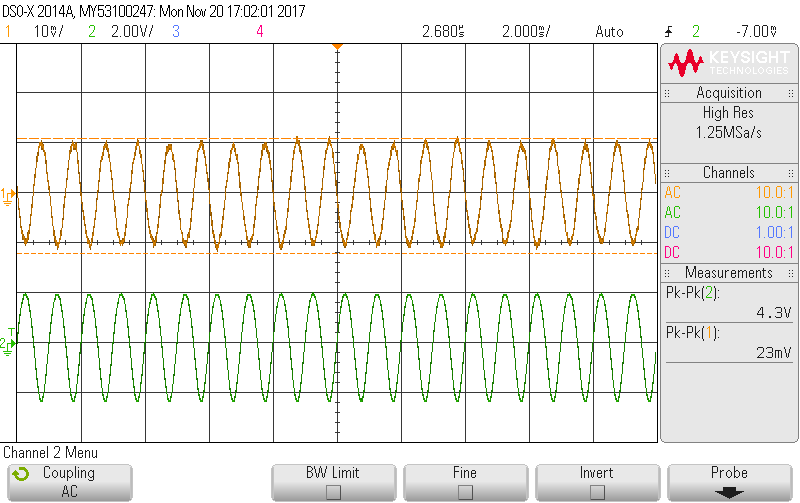
\includegraphics[width=\textwidth]{CEE}

\caption{Testing of the Common Emitter Amplifier}
\label{CEE}
\end{figure}
\subsubsection{Band Pass Filter}
To construct the band pass filter the Inductor must first be made. It was calculated that the required inductor would be made of 61 turns. This Inductor was created and its inductance was measured using an LCR meter. The desired inductance is $11.3mH$ however the inductance was measured as $11.9mH$, to reduce this turns were removed and the Inductor re measured until its inductance was equal to $11.3mH$. This was achieved with 56 turns. The circuit was then constructed on the circuit board according to the circuit diagram shown in Figure \ref{BPF}. Once completed the filter was characterised between $1Hz$ and $5kHz$ with a $2V Pk-Pk$ sine wave input shown in figure \ref{BandPassFilter}. 

\begin{figure}[!h]
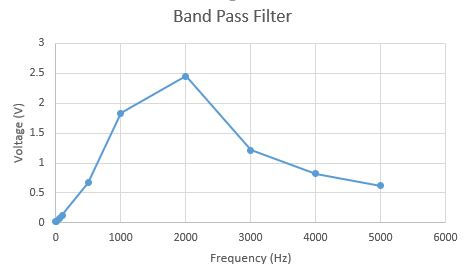
\includegraphics[width= \textwidth]{BPF}
\caption{Characterisation of Band Pass Filter}
\label{BandPassFilter}
\end{figure}
\subsubsection{Signal Rectifier}
The circuit shown in figure \ref{RecDia} was constructed on the circuit board and was then tested as shown in figure \ref{Rectifier} with a $1.5kHz$ $5V$ sine wave.





\begin{figure}[!h]
\includegraphics[scale= 0.75]{rectifierdia}
\caption{Rectifier Circuit Diagram}
\label{RecDia}
\end{figure}

\begin{figure}[!h]
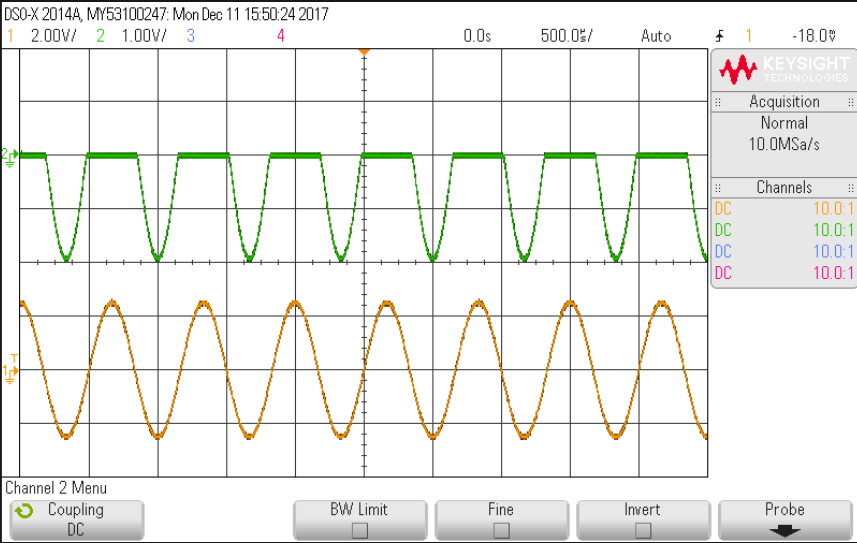
\includegraphics[scale= 0.5]{rectifier}
\caption{Rectifier analysis}
\label{Rectifier}
\end{figure}
\subsubsection{Low Pass Filter}
The Low Pass Filter was constructed on the circuit board according to the circuit diagram shown in figure \ref{LPF}. After the circuit was constructed it was tested by inputting a $1V Pk-Pk$ sine wave as shown in figure \ref{LPFscope}. The filter was then characterised between $1Hz$ and $1kHz$ with a $1V Pk-Pk$ input sine wave shown in figure \ref{LPFchar}. The filter has a $-3dB$ cutoff point at $F_c \approx 80Hz$ 

\begin{figure}
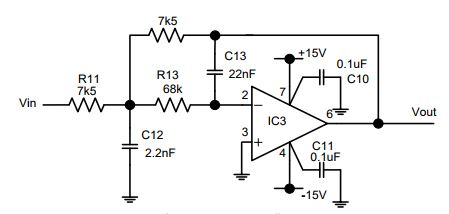
\includegraphics[width=\textwidth]{LPF}
\caption{Low Pass Filter Circuit Diagram}
\label{LPF}
\end{figure}

\begin{figure}[!h]
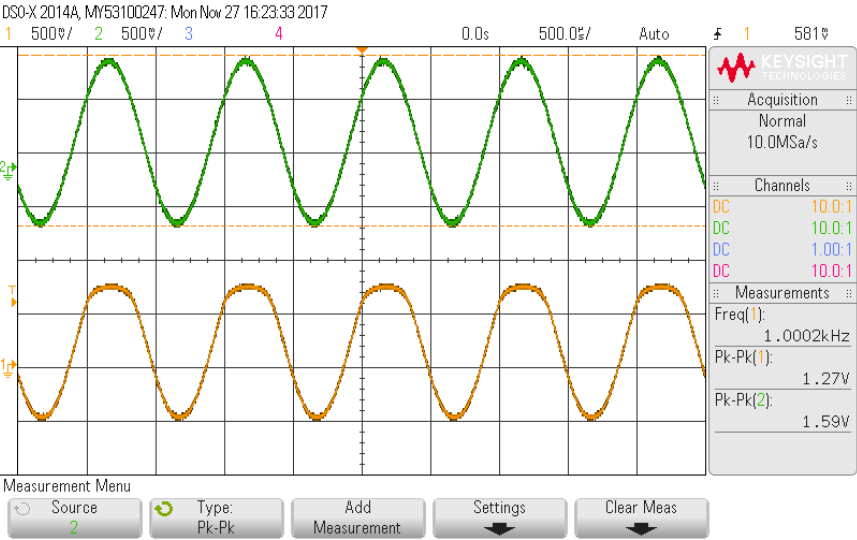
\includegraphics[width =\textwidth]{lpfilter}
\caption{Low Pass Filter input \& output}
\label{LPFscope}
\end{figure}

\begin{figure}[!h]
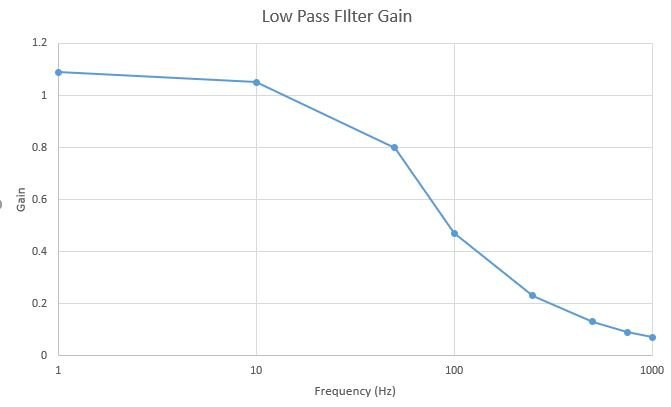
\includegraphics[width = \textwidth]{LPFchar}
\caption{Low Pass Filter Characterisation}
\label{LPFchar}
\end{figure}

\subsubsection{PIC Microcontroller}
The Microcontroller circuit was constructed according to the circuit diagram shown in figure \ref{PIC}. The PIC was then programmed with the code shown in the design phase shown in figure \ref{code}.

\begin{figure}[!h]
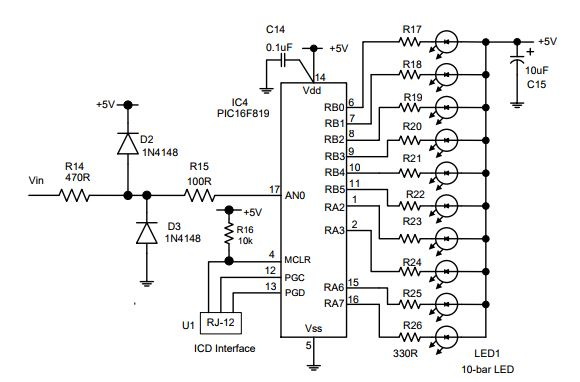
\includegraphics[width = \textwidth]{PIC}
\caption{PIC Microcontroller circuit diagram}
\label{PIC}
\end{figure} 

\subsubsection{Final Test}
Once all parts of the circuit were connected together the meter was tested by playing a $1.5kHz$ tone through a speaker from a signal generator near the meter and observing the LED's.







\section{Analysis}
\subsection{Common Emitter Amplifier}
The Common Emitter Amplifier is used to amplify the low level signals coming from the microphone. This amplifier is used due to multiple attributes of the amplifier, namely, high input impedance, class A operation to prevent distortion and high single stage gain.

\subsubsection{Input Impedance}
The high input impedance is needed as the microphone is a high impedance device and to allow maximum power transfer between the microphone and the amplifier $Z_{mic} \approx Z_{amp}$. If this were not the case the already small signal from the microphone would be reduced even more due to internal losses in the internal series impedance of the microphone. The input impedance of the amplifier can be calculated by looking at what impedance the input sees looking in to the input, this is ,$R1$,$R2$ and the impedance lookin in to the base all in paralell \cite{ArtElectronics}. $R1 = 270k\Omega$,$R2 = 40k\Omega$ and the impedance looking in to the base is $h_{fe} \times R_E$ as $h_{fe}$ is equal to $\beta$ \cite{ArtElectronics} $265k\Omega= 787(R_4)\Omega \times 337(\beta)$.
this works out to be  

\begin{center}
\Huge

$Z_{in}= (\frac{1}{270\times 10^{3}} +\frac{1}{40\times 10^{3}} + \frac{1}{265 \times 10^{3}} )^{-1} \approx 31k\Omega$



\end{center}
The input capacitor $C_1 = 10\mu F$ is in series with the input impedance of $31k\Omega$, the capacitor also forms a high pass filter with the input impedance 
\begin{center}
\Huge

$F_c = \frac{1}{2\pi RC} = 0.5Hz$



\end{center}
\cite{ArtElectronics}
As the $3dB$ cut-off point is $0.5Hz$ almost all signal energy will be well above this point so the attenuation of this high pass filter can be ignored as it is negligible at frequencies of interest.
\subsubsection{Output Impedance}
The output impedance of the amplifier is calculated as the collector resistor in parallel with the resistance looking in to the collector. The resistance of the collector resistor is know as $3.9k\Omega$ and the resistance looking in to the collector is te resistance of the transistor and the emitter resistor in series. As the transistor can be modelled as a current source there is a current source in series with $R_E$. A current source has impedance $\approx \infty$. The output impedance is therefore the $3.9k\Omega$ resistor in parallel with a near infinite resistance so $Z_{out} \approx 3.9K\Omega$. This output impedance is low enough to allow good signal transfer to the next stage as the input impedance to the next stage is at lowest $4.7k\Omega$ which is higher than the output impedance.
\subsubsection{Biasing}
The transistor is biased with $R1$ and $R2$, These resistors are used to provide a constant quiescent current through the base and in turn from Collector to Emitter. This is done so that in the steady state the voltage at the collector with respect to ground is $\approx 7.5V$. This is done to allow the amplifier to produce positive and negative voltage swings. Without biasing the collector would be at $15V$ in the steady state due to no quiescent current flowing through $R1$ so no voltage drop across it. Due to this node being at $15V$ the amplifier can only produce a negative voltage swing as this node is already at the highest voltage in the circuit so cannot go higher. If however this point is at $7.5V$ half way between ground and Vcc then it can swing positive and negative in equal amounts. The capacitor $C_2$ is used to remove the DC offset of the output so as to make the signal centred around $0V$ instead of $7.5V$.\newline
      The resistors are chosen of values to allow the desired amount of quiescent  current flows through the base. This is done by using a voltage divider configuration. This configuration however causes a design challenge that the current flowing through $R2$ must be about ten times grater than the current flowing through the base to prevent this "load" on the voltage divider from lowering the voltage at its mid point and producing incorrect biasing.    
\subsubsection{Emitter Capacitor}
The emitter capacitor $C_3$ is chosen to allow stable biasing of the amplifier. Due to the relatively low emitter resistor of $787\Omega$ the emitter voltage across $R4$ can become small when compared to the voltage drop $V_{BE}$ \cite{ArtElectronics}. This leads to instability in the biasing and the quiescent voltage at the collector as $V_{BE}$ varies with temperature. This change in $V_{BE}$ with temperature causes changes in the base current with temperature. To solve this problem and still have an amplifier with high gain(Necessitating a low $R_E$) a capacitor is placed in parallel with $R_E$. The capacitor is chosen so as to create the effect of a low impedance $R_E$ at signal frequencies but the DC biasing signal only sees a high impedance $R_4$(as the capacitor has infinite impedance at DC),so as to prevent the instability aforementioned. The capacitor must be chosen so that at signal frequencies its impedance is low compared to $r_e$ the resistance between base and emitter\cite{ArtElectronics}. In this circuit the DC biasing signal sees $\beta \times 787\Omega = 265k\Omega$ as the resistance looking in to the base, however at a frequency of $1kHz$ an input signal looking in to the base would see $787\Omega$ in parallel with $\approx 0.5\Omega$ times $h_{fe}$ or about $168\Omega$. This allows a low effective emitter resistor without the insatiability that this causes.  

\subsection{Band Pass Filter}   
The band pass filter section is formed from a parallel resonant circuit and a non inverting amplifier.

\subsubsection{Parallel Resonant Circuit}
The Parallel Resonant Circuit is formed form $R6,L1\&C5$. The Parallel Resonant Circuit has a frequency response of $0\Omega$ resistance at DC and infinite frequency as at DC the inductor is a short to ground and at infinite frequency the Capacitor is a short to ground. At the resonant frequency current flows backwards and forwards between the capacitor and inductor in phase with the input signal, this voltage opposes the input signal so no current can flow through the capacitor or inductor, as there is a voltage across the components but no current is flowing then the components must have infinite impedance from the perspective of the input signal. No current is drawn from the supply as $I_l = -I_C$ so $I_L + I_C = 0$ at resonance. For this particular circuit the resonant frequency is equal to

\begin{center}
\Huge

$F=\frac{1}{2\pi\sqrt{LC}} = 1.5kHz$



\end{center}
The circuit also has a property called $Q$. The $Q$ factor is a representation of how damped the circuit is. Damping is a measure of the loss of energy from the circuit. A parallel LC circuit with ideal inductors and capacitors would have a $Q = \infty$ as no energy is lost from the circuit and the resonant oscillations would continue forever. The higher the Q of the circuit the sharper the peak of resonance is meaning that a high Q circuit would transition form low impedance at frequencies not equal to the resonant to high impedance at the resonant frequency very quickly and then transition back to low impedance very quickly. The $Q$ factor for this circuit is given by. 




\begin{center}
\Huge

$Q= \omega_0RC = 2.07$



\end{center}


\begin{figure}[!h]
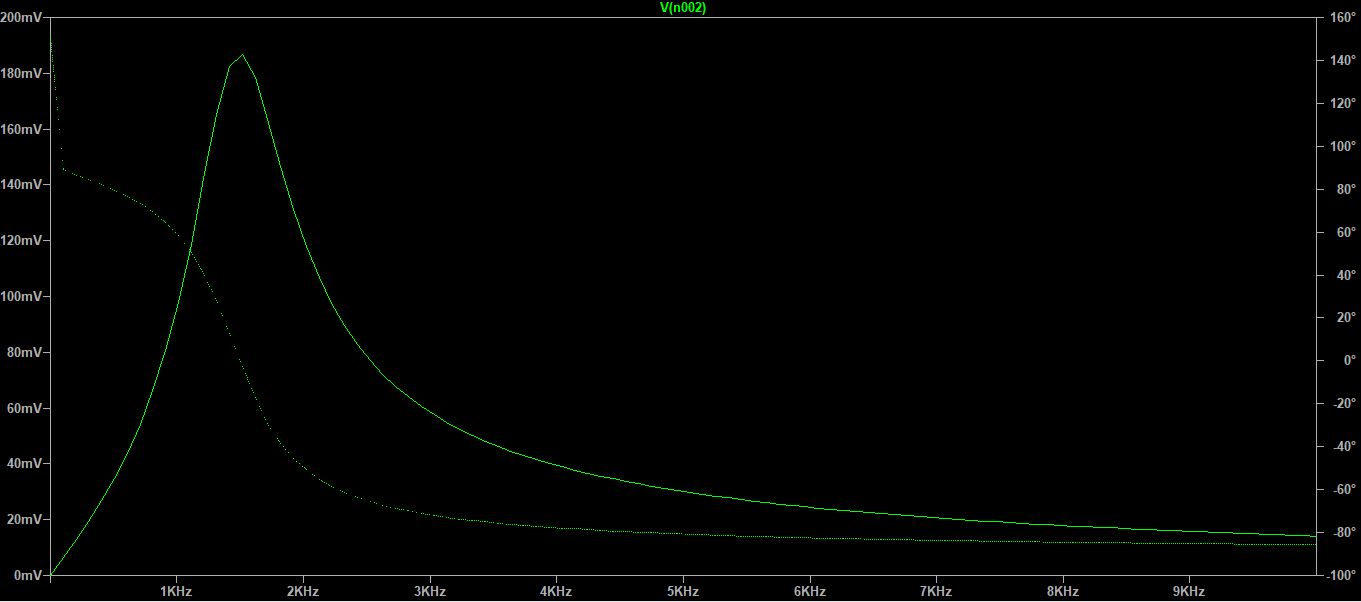
\includegraphics[width=\textwidth]{BPFgraph}
\caption{Voltage against frequency for band pass filter}
\label{BPFgraph}
\end{figure}










   
This means that the bandwidth of the filter is $723Hz$ as bandwidth is equal to the resonant frequency divided by the $Q$ factor. The $3dB$ pass band for this filter is $1140Hz$ to $1860Hz$. This however is not precise as the resonant circuit is also damped by the output impedance of the Common Emitter amplifier in series with $R_5$ and the impedance of the Capacitor $C_2$. This however is much higher than the $220\Omega$ resistor that is designed to damp the circuit so can be ignored as it is in parallel with the damping resistor. It can be seen from Figure \ref{BPFgraph} that the signal is phase shifted positively below the resonant frequency and negatively above the resonant frequency with 0 phase shift     at the resonant frequency. This is because below the resonant frequency the circuit appears inductive and above the resonant frequency the circuit appears capacitive.The output of the filter is then fed in to a non inverting amplifier as this has a very high input impedance to prevent further loading of the resonant circuit. The amplifier has a gain given by
\begin{center}
\Huge

$G= 1+ \frac{R_8}{R_7}\approx 38$



\end{center}
\subsection{Rectifier}
The rectifier section is formed by a Diode to allow current to flow only in one direction and a unity gain buffer to provide a low impedance drive to the next stage
\subsubsection{Diode}
The Diode only allows current to flow in one direction. This diode only allows negative voltages to be passed, this can be seen in figure \ref{Rectifier} as the output only has negative peaks but the input has both negative and positive peaks but the diode removed them.
 

\section{Conclusion}

\printbibliography

\end{document}
